\cleardoublepage
%\newpage
%\thispagestyle{empty}
\mbox{}

\chapter{Tecnología de las FPGAs}
\label{ch:chapter3}

Las FPGAs (Field Programmable Gate Arrays) \cite{biblio:Tesis_Carlos} son dispositivos hardware programables y reconfigurables de bajo consumo que ofrecen un gran equilibrio entre flexibilidad y eficiencia, motivos por los cuales han sido elegidas para la implementación del algoritmo en este trabajo. Consisten en una matriz de bloques lógicos o LB (Logic Blocks) y una red de interconexión que pueden ser configurados haciendo uso de dispositivos anti–fuse \cite{biblio:Tesis_Carlos} o mediante un mapa de bits (bitstream) \cite{biblio:bitstream} según la funcionalidad que se requiera.

Los LBs interconectados mediante esa red contienen típicamente uno o varios circuitos combinacionales programables Look-Up Table (LUT), uno o varios biestables, lógica adicional y las celdas de memoria SRAM requeridas para la configuración de todos los elementos. Las tareas de entrada/salida se realizan en la periferia del dispositivo mediante LBs o mediante bloques específicos denominados Input–Output–Blocks (IOBs). La figura~\ref{fig:modelo generico fpga} \cite{biblio:Tesis_Carlos} muestra la estructura interna simplificada de una FPGA.

\begin{figure}
  \centering
    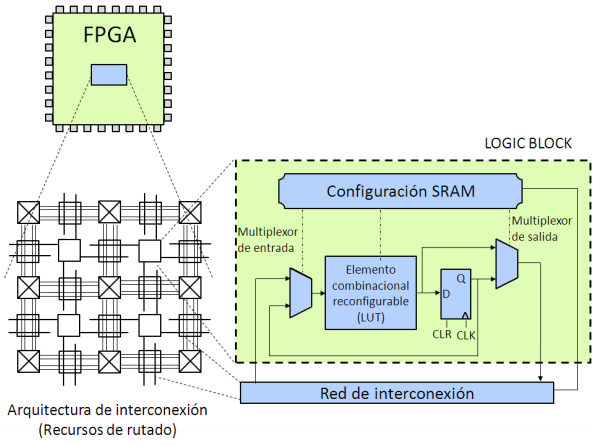
\includegraphics[width=0.8\textwidth]{Imagenes/ModeloGenericoFPGA.png}
  \caption{Modelo genérico de una FPGA.}
  \label{fig:modelo generico fpga}
\end{figure}

%[CarlosIni]Hay que contar que las FPGAs actuales tienen recursos hetereogéneos como memoerias, DSPs y hasta procesadores.[CarlosFin]

Actualmente, se integran también de forma habitual recursos heterogéneos como bloques de memoria RAM dedicada \cite{biblio:ram_dedicada}, multiplicadores, interfaces para periféricos, DSPs (Digital Signal Processor) e incluso microprocesadores. Con la integración de estos elementos arquitectónicos en FPGAs que disponen de una sección de lógica programable por el usuario surge el concepto de Arquitecturas Híbridas \cite{biblio:bitstream}.

El diseño con FPGAs se lleva a cabo mediante un proceso automático conocido como síntesis de alto nivel. Los algoritmos o las tareas deben ser descritos en un lenguaje de alto nivel que esté directamente relacionado con elementos hardware para su fácil traducción a un circuito. En los últimos años se ha utilizado mayormente los lenguajes de descripción hardware (HDL, Hardware Description Language), entre los que destacan Verilog y VHDL.

El primer paso para sintetizar una tarea a hardware es describir el algoritmo en alguno de los HDLs disponibles (por ejemplo, VHDL). El siguiente paso es determinar qué tipo de bloques hardware son necesarios y cómo están conectados entre sí para después, en el tercer paso, asignar bloques básicos configurables concretos de la FPGA (CLBs) y el rutado de señales entre ellos. En el cuarto paso del proceso se obtiene el mapa de bits de configuración necesario para que los LBs utilizados en el diseño del circuito realicen cada uno la funcionalidad necesaria. Por último, es necesario escribir dicho mapa de bits en la memoria de configuración del dispositivo.

Las ventajas que presentan las FPGAs son el aumento de la velocidad de procesamiento \cite{biblio:TFG_Esquembri}, ya que, además de presentar la posibilidad real de paralelización, una ejecución hardware es habitualmente más rápida que el código software; la reducción del consumo, ya que se pueden aplicar técnicas para evitar el consumo innecesario; flexibilidad \cite{biblio:embedded}, ya que existe la posibilidad de reconfigurar los elementos básicos; y el coste reducido debido al aumento de su popularidad y a los avances en la fabricación de su tecnología.

Por otra parte, existen dos aspectos importantes a tener en cuenta \cite{biblio:TFG_Esquembri}: uno es el rutado de las señales, ya que el obtenido tras la compilación no suele ser el más eficiente y suele ser necesaria una revisión manual por parte del diseñador. La solución por la que se opta para mejorar este aspecto es el diseño 3D \cite{biblio:diseno3d}. El otro aspecto es el elevado tiempo de configuración debido al gran tamaño que suele tener el mapa de bits necesario. Ya se están dirigiendo numerosos esfuerzos en nuevas arquitecturas o tecnologías que permitan paliar este efecto.

%\newpage
%\thispagestyle{empty}
%\mbox{}